\section{Locality-Sensitive Hashing (LSH)}

\subsection{Introduction to LSH}

Locality-Sensitive Hashing (LSH) is a hashing-based approach for approximate nearest neighbor (ANN) search. The concept of LSH was first introduced by Indyk and Motwani in 1998 \cite{Indyk-Motwani-1998} and later improved and generalized by Gionis, Indyk, and Motwani in 1999 \cite{Gionis-Indyk-Motwani-1999}.

The key idea of LSH is to design hash functions such that similar objects are mapped to the same bucket with high probability, while dissimilar objects are unlikely to collide. This property allows sublinear query time, as the search can be restricted to the elements stored in the buckets corresponding to the query point \cite{Gionis-Indyk-Motwani-1999}.

LSH significantly improved running time over previous methods for searching in high-dimensional spaces based on hierarchical tree decompositions \cite{Gionis-Indyk-Motwani-1999}. Although more recent graph-based and quantization-based methods, such as HNSW or IVF-PQ, often outperform LSH in practice, it remains a foundational algorithm with strong theoretical guarantees and continues to influence modern research in approximate nearest neighbor search.

\subsection{Description of LSH}

To simplify the presentation, the algorithm is described \cite{Gionis-Indyk-Motwani-1999} under two assumptions: (i) distances are measured with the $l_1$ norm, and (ii) all coordinates of the data points are positive integers. After these transformations, the minimum interpoint distance is guaranteed to be one.

Let $C$ be the largest coordinate value in all points in $P$. Each point 
$p = (x_{1}, \ldots, x_{d})$ is conceptually mapped to a binary vector in dimension $d' = C \cdot d$ by concatenating the unary representations of its coordinates:
\[
v(p) = \text{Unary}_{C}(x_{1}) \;\Vert\; \dots \Vert\; \text{Unary}_{C}(x_{d}),
\]
where $\text{Unary}_{C}(x)$ is a binary string of $x$ ones followed by $C - x$ zeros. This mapping preserves distances: the $l_1$ distance in the original space equals the $d_H$ distance in the Hamming space $H^{d'}$. In practice, the unary expansion is not materialized explicitly; it is used only as a conceptual framework for defining the algorithms.

\newpage

\paragraph{Hash Functions}

The LSH scheme uses $l$ different hash tables, each associated with its own hash function $g_{j}$, for $j = 1, \dots, l$. For each hash table, the function $g_{j}$ is defined by selecting $k$ coordinates uniformly at random (with replacement) from $\{1, \dots, d'\}$ and projecting the binary vector $v(p)$ onto these positions, producing $g_{j}(p)$. The parameter $k$ is chosen to maximize the probability that a point close to a query $q$ falls into the same bucket as $q$, while minimizing the probability that a distant point collides in the same bucket. Each point $p \in P$ is then stored in the corresponding bucket $g_{j}(p)$ across all $l$ tables (Figure~\ref{fig:lsh-1}).

Since the number of buckets can be very large, a second level of hashing is used to compress them into a hash table of fixed size $M$, with each bucket limited to a maximum capacity of $B$ \cite{Gionis-Indyk-Motwani-1999}. The selection of the parameters $l$ and $k$ is discussed in the next section.

\begin{figure}[H]
    \centering
    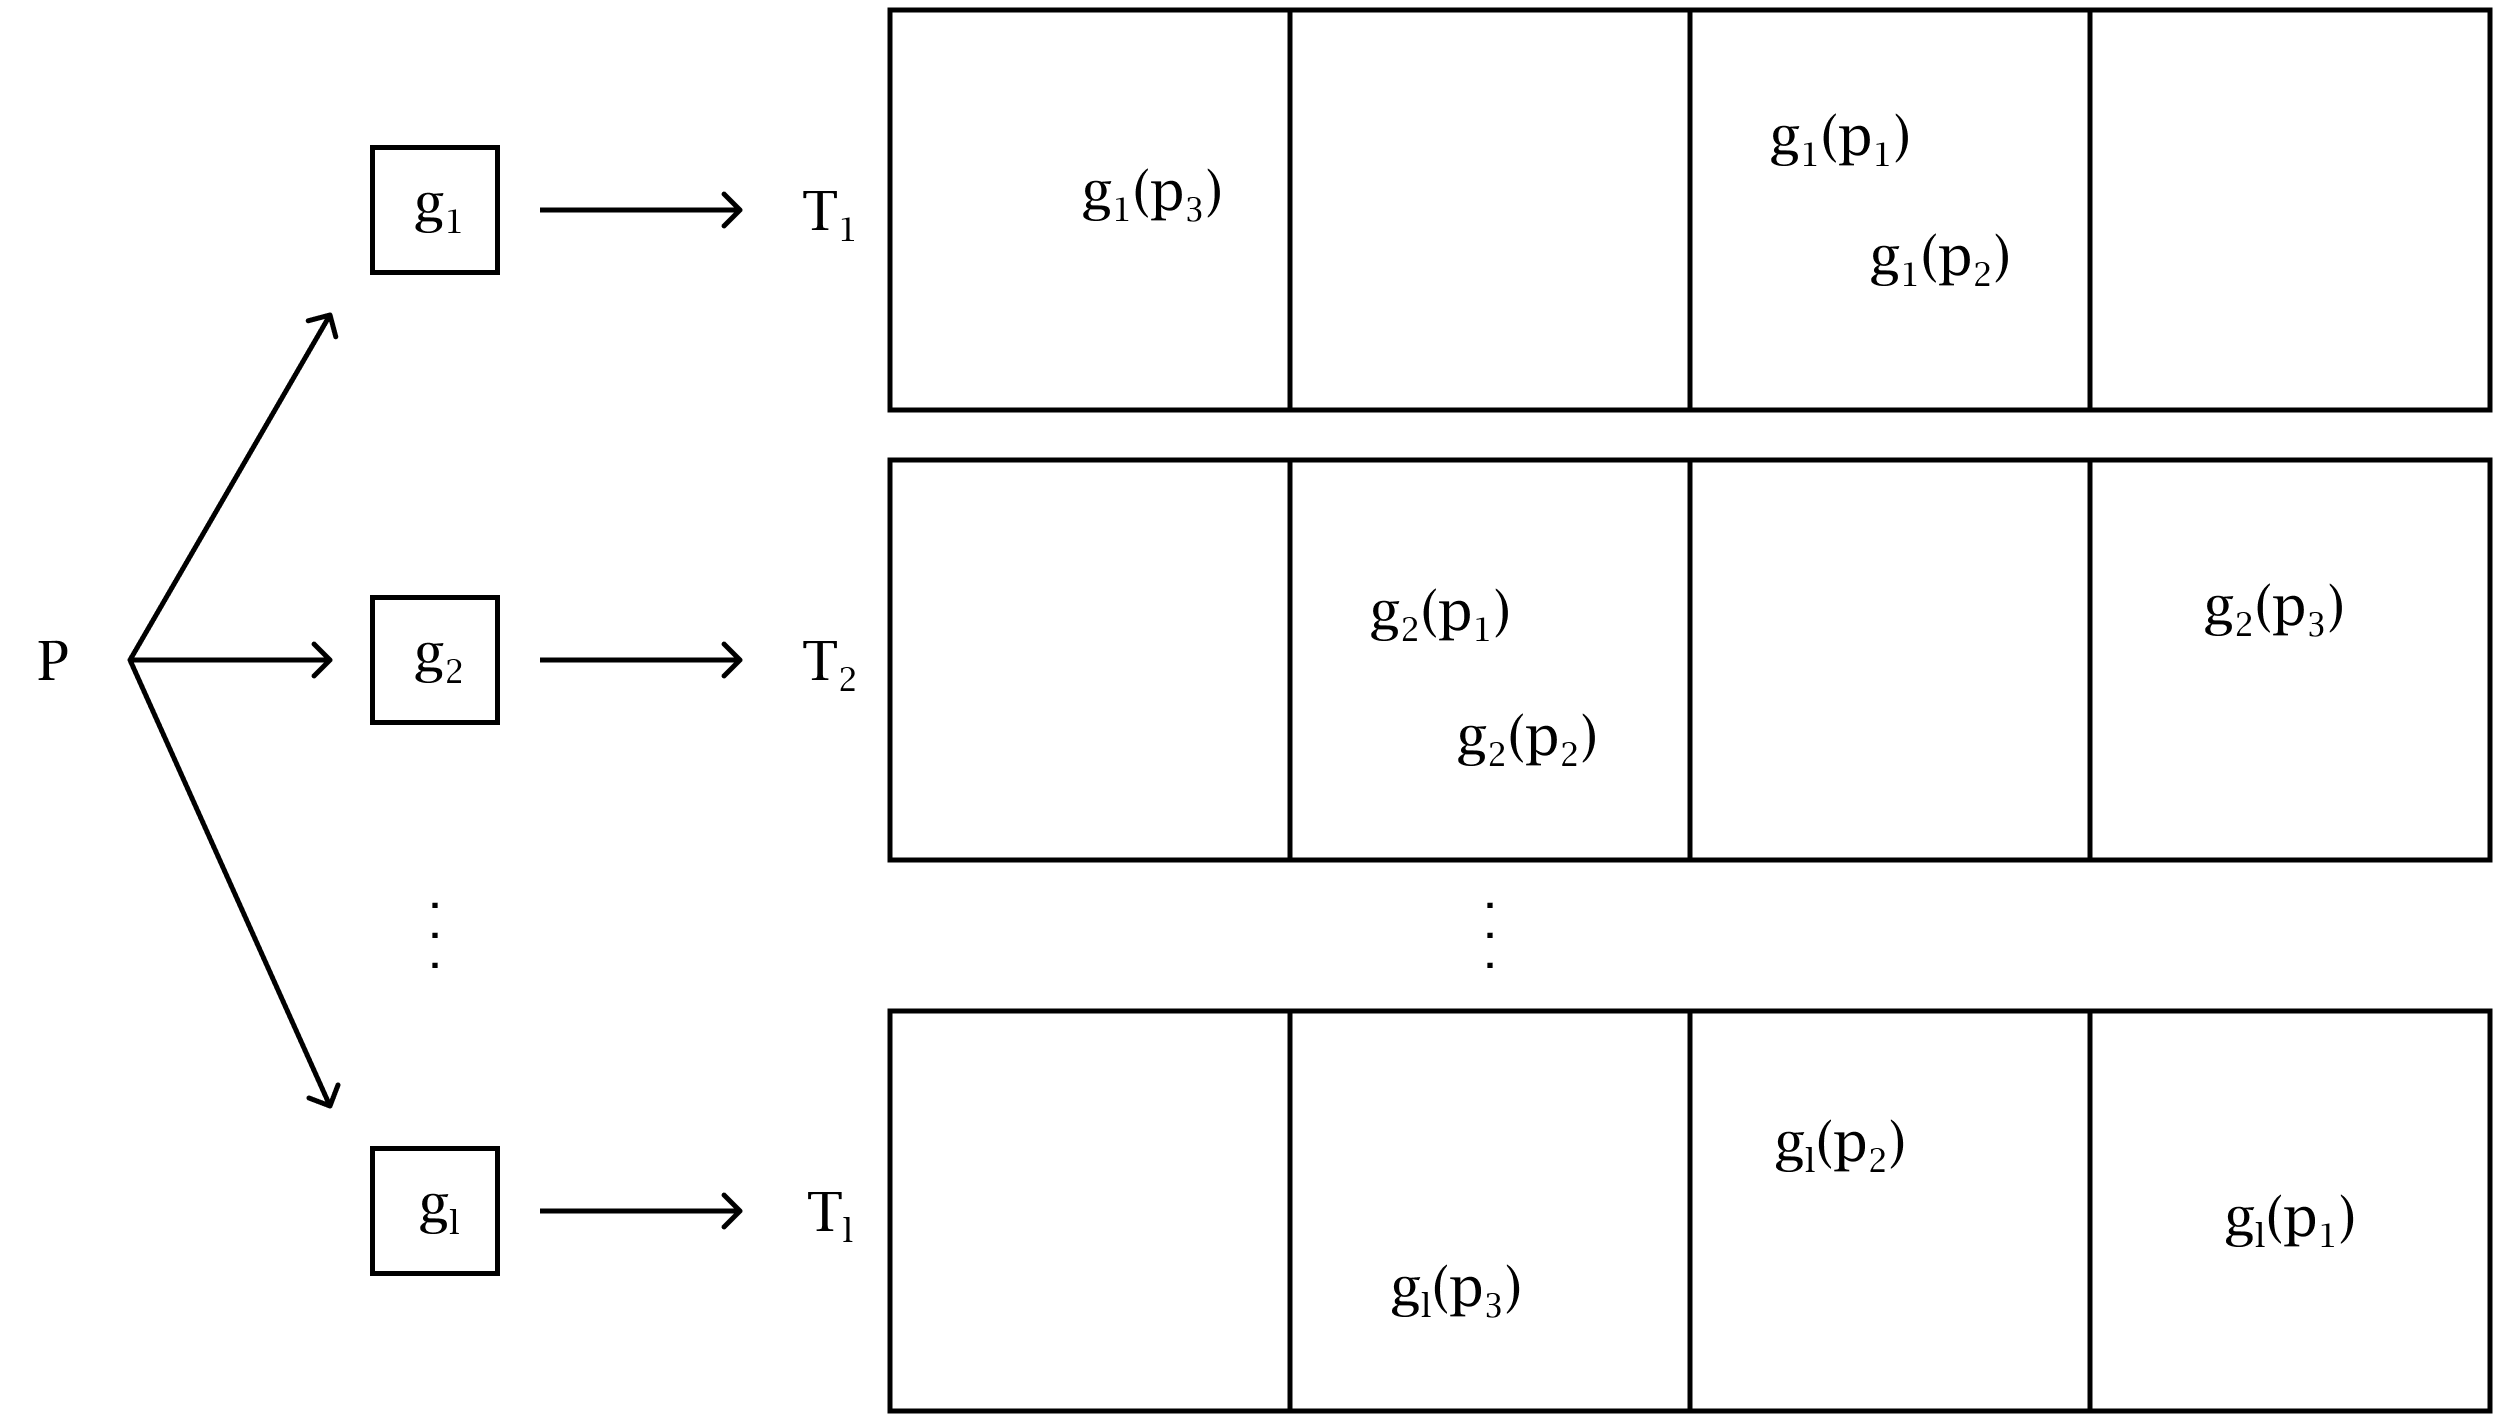
\includegraphics[width=0.9\textwidth]{chapters/algorithms/lsh/figures/hashing.png}
    \caption{LSH hashing process. Each data point $p \in P$ is projected via hash functions $g_j$ into buckets across $l$ hash tables.}
    \label{fig:lsh-1}
\end{figure}

\subsubsection{Indexing}

The indexing stage (Algorithm~\ref{alg:lsh-1}) constructs the $l$ hash tables and distributes the dataset points into the appropriate buckets:

\begin{algorithm}[H]
    \caption{BUILD-INDEX \cite{Gionis-Indyk-Motwani-1999}}
    \label{alg:lsh-1}
    \begin{algorithmic}[1]
        \Require points $P$, number of hash tables $l$
        \Ensure hash tables $T$
    
        \For{$i \gets 1 \dots l$}
            \State generate random hash function $g_i(\cdot)$ and initialize hash table $T_i$
            
            \For{each $p \in P$}
                \State store point $p$ in bucket $g_i(p)$ of hash table $T_i$
            \EndFor
        \EndFor
    \end{algorithmic}
\end{algorithm}

\subsubsection{Querying}

To answer a query, the algorithm (Algorithm~\ref{alg:lsh-2}) hashes the query point $q$ into each of the $l$ tables, retrieves candidate points from the corresponding buckets, and returns the $k$ nearest neighbors from the candidate set:

\begin{algorithm}[H]
    \caption{K-NN-SEARCH \cite{Gionis-Indyk-Motwani-1999}}
    \label{alg:lsh-2}
    \begin{algorithmic}[1]
        \Require $l$ hash tables $T$, query point $q$, number of nearest neighbors $k$
        \Ensure up to $k$ approximate nearest neighbors of $q$
        
        \State $S \gets \emptyset$ \Comment{candidate set}
        
        \For{$i \gets 1 \dots l$}
            \State $S \gets S \cup \{$points in bucket $g_i(q)$ of hash table $T_i\}$
        \EndFor
        
        \State \Return up to $k$ nearest neighbors of $q$ in $S$
    \end{algorithmic}
\end{algorithm}

\subsection{Analysis of LSH}

The main intuition behind LSH is that the probability of two points colliding in the same hash bucket decreases as the distance between them increases, which is formalized as follows \cite{Gionis-Indyk-Motwani-1999}. Let $D(\cdot, \cdot)$ be a distance function on a set $S$, and for any $p \in S$ let $\mathcal{B}(p, r)$ denote the set of elements from $S$ within distance $r$ from $p$. A family $\mathcal{H} = \{h: S \to U\}$ is called $(r_1, r_2, p_1, p_2)$-sensitive for $D(\cdot, \cdot)$ if for any $p, q \in S$:

\begin{itemize}
    \item If $p \in \mathcal{B}(q, r_1)$, then $\Pr_{\mathcal{H}}[h(q) = h(p)] \ge p_1$.
    \item If $p \notin \mathcal{B}(q, r_2)$, then $\Pr_{\mathcal{H}}[h(q) = h(p)] \le p_2$.
\end{itemize}

For a locality-sensitive family to be useful, it must hold that $p_1 > p_2$ and $r_1 < r_2$. This ensures that points close to the query are likely to collide in a hash bucket, while distant points are unlikely to.

\paragraph{Hamming Locality-Sensitive Family}

When the distance function is the Hamming distance, the family of projections on one coordinate is locality-sensitive. Specifically, let $S = H^{d'}$ and $D(p, q) = d_H(p, q)$ for $p, q \in H^{d'}$. Then for any $r, \epsilon > 0$, the family
\[
\mathcal{H}_{d'} = \Bigl\{ h_i : h_i\Bigl((b_1, \dots, b_{d'})\Bigr) = b_i, \; i = 1, \dots, d' \Bigr\}
\]
is 
\[
\Big(r, r(1 + \epsilon), 1 - \frac{r}{d'}, 1 - \frac{r(1 + \epsilon)}{d'}\Big)\text{-sensitive}.
\] 
That is, points within distance $r$ collide with probability at least $1 - r/d'$, while points farther than $r(1 + \epsilon)$ collide with probability at most $1 - r(1 + \epsilon)/d'$ \cite{Gionis-Indyk-Motwani-1999}.

\paragraph{Arbitrary Locality-Sensitive Family}

The algorithm can be generalized to any locality-sensitive family $\mathcal{H}$. In this case, each hash function is defined as
\[
g_i(p) = (h_{i_1}(p), \dots, h_{i_k}(p)),
\]  
where $h_{i_1}, \dots, h_{i_k}$ are randomly chosen from $\mathcal{H}$ with replacement. As before, $l$ such functions $g_1, \dots, g_l$ are constructed to build $l$ hash tables \cite{Gionis-Indyk-Motwani-1999}.

\paragraph{Correctness via the $(r, \epsilon)$-Neighbor Problem}

Formally, the algorithm is shown \cite{Gionis-Indyk-Motwani-1999} to correctly solve the so-called $(r, \epsilon)$-Neighbor problem, which asks whether there exists a point $p$ within a fixed distance $r_1 = r$ of the query $q$, or whether all points are at least distance $r_2 = (1 + \epsilon)r$ away. In particular, the LSH algorithm solves this problem for a proper choice of parameters $k$ and $l$, depending on $r$ and $\epsilon$. More precisely, for the set of points $P' \subseteq P$ farther than $r_2$ from $q$, the algorithm correctly solves the $(r, \epsilon)$-Neighbor problem if the following two properties hold:

\begin{itemize}
    \item[\textbf{P1}] If there exists a point within distance $r_1$ of the query, then at least one of the hash functions $g_1, \dots, g_l$ maps it to the same bucket as the query.
    \item[\textbf{P2}] The total number of hash buckets pointed to by the query that contain only points from $P'$ is bounded by $c \cdot l$, for some constant $c$.
\end{itemize}

Intuitively, P1 ensures that close points are likely to be retrieved by the query, while P2 guarantees that the number of far points incorrectly considered is limited, keeping the search efficient. As proven in \cite{Gionis-Indyk-Motwani-1999}, by choosing the parameters:

\[
k = \log_{\frac{1}{p_2}} \frac{n}{B}, \quad 
l = \left( \frac{n}{B} \right)^\rho, \quad 
\rho = \frac{\ln \frac{1}{p_1}}{\ln \frac{1}{p_2}}
\]

both properties P1 and P2 hold with probability at least $1/2 - 1/e \ge 0.132$, ensuring the correctness of the LSH algorithm.\newline

When instantiated for the Hamming locality-sensitive family, it can be shown that
\[
\rho \le \frac{1}{1 + \epsilon}
\]
under the assumption that $r < d'/\ln n$ which can be easily satisfied. Thus, the expected query time of the LSH algorithm is sublinear in the number of points $n$. Specifically, for a dataset of $n$ points in dimension $d$, the query time is $O\bigl(d \cdot n^{1 / (1 + \epsilon)}\bigr)$ \cite{Gionis-Indyk-Motwani-1999}.

\paragraph{Connection to the $\epsilon$-NNS Problem}

While the $(r, \epsilon)$-Neighbor problem is central for the theoretical analysis of LSH, in practice the main objective is to solve the $\epsilon$-Nearest Neighbor Search ($\epsilon$-NNS) problem. This problem can be reduced to a sequence of $(r, \epsilon)$-Neighbor instances for different values of $r$, specifically $r_0, r_0(1 + \epsilon), r_0(1 + \epsilon)^2, \dots, r_{\max}$, where $r_0$ and $r_{\max}$ denote the smallest and the largest possible distance between the query and the dataset, respectively \cite{Gionis-Indyk-Motwani-1999}. By testing successive $(r, \epsilon)$-Neighbor instances for increasing values of $r$, one can identify the smallest radius at which a neighbor is detected.

However, empirical evidence suggests that in most cases a single fixed value of $r$ is sufficient, since the distribution of distances between queries and the dataset typically depends more on the intrinsic properties of the data than on the particular query point. Consequently, in practice a fixed choice of $r$ is often adopted, which also fixes the values of $k$ and $l$ for the entire dataset \cite{Gionis-Indyk-Motwani-1999}.